\documentclass[12pt,a4paper,openany]{report}
\usepackage[T1]{fontenc}
\usepackage{lmodern}
\usepackage[margin=1in]{geometry}
\usepackage{tabularx}
\usepackage{booktabs}
\usepackage{titlesec}
\titlespacing*{\chapter}{0pt}{0pt}{18pt}
\titlespacing*{\section}{0pt}{8pt}{2pt}
\usepackage{tikz}
\usetikzlibrary{positioning,calc,arrows.meta}

\definecolor{apexfill}{HTML}{DCE6F1}
\definecolor{apexline}{HTML}{2F5496}
\definecolor{subfill}{HTML}{F2F2F2}
\definecolor{subline}{HTML}{666666}
\definecolor{cabfill}{HTML}{BDD7EE}
\definecolor{cabline}{HTML}{1F4E79}
\definecolor{mosfill}{HTML}{FCE4D6}
\definecolor{mosline}{HTML}{C55A11}
\definecolor{cmred}{HTML}{C00000}
\hyphenation{Chancellorship direction}

\tikzset{
  hroot/.style={draw=apexline, fill=apexfill, rounded corners=4pt,
                line width=0.8pt, text width=3.6cm, align=center,
                minimum height=1.25cm, font=\bfseries,
                execute at begin node={\hyphenpenalty=10000\relax}},
  hlvl/.style={draw=apexline!70, fill=apexfill!60, rounded corners=3pt,
               line width=0.7pt, text width=3.2cm, align=center,
               minimum height=1.1cm, font=\small,
               execute at begin node={\hyphenpenalty=10000\relax}},
  hsub/.style={draw=subline, fill=subfill, rounded corners=3pt,
               line width=0.6pt, text width=2.7cm, align=center,
               minimum height=1.0cm, font=\small},
  hleaf/.style={draw=subline, fill=subfill!75, rounded corners=3pt,
                line width=0.6pt, text width=2.7cm, align=center,
                minimum height=0.9cm, font=\footnotesize,
                execute at begin node={\hyphenpenalty=10000\relax}},
  cabbox/.style={draw=cabline, fill=cabfill, rounded corners=3pt,
                 line width=0.8pt, text width=3.4cm, align=center,
                 minimum height=1.1cm, font=\bfseries\small},
  mosbox/.style={draw=mosline, fill=mosfill, rounded corners=3pt,
                 line width=0.8pt, text width=3.4cm, align=center,
                 minimum height=1.1cm, font=\bfseries\small},
  minbox/.style={draw=subline, fill=subfill!70, rounded corners=2pt,
                 line width=0.5pt, text width=3.4cm, align=center,
                 minimum height=0.9cm, font=\scriptsize,
                 execute at begin node={\hyphenpenalty=10000\relax}},
  hlink/.style={draw=black!65, line width=0.7pt},
  fnbox/.style={draw=apexline!55, fill=apexfill!45, rounded corners=3pt,
                line width=0.6pt, text width=5.5cm, align=left,
                minimum height=2.6cm, font=\footnotesize, inner sep=6pt,
                execute at begin node={\hyphenpenalty=10000\relax}},
  elecbox/.style={draw=apexline!70, fill=apexfill!45, rounded corners=3pt,
                  line width=0.7pt, text width=10.8cm, align=center,
                  minimum height=1.45cm, font=\small,
                  execute at begin node={\hyphenpenalty=10000\relax}},
  secbox/.style={draw=apexline!55, fill=apexfill!30, rounded corners=3pt,
                 line width=0.6pt, text width=7.3cm, align=left,
                 minimum height=4.0cm, font=\scriptsize, inner sep=7pt,
                 anchor=north,
                 execute at begin node={\hyphenpenalty=10000\relax}}
}

\begin{document}

% ---------------------------------------------------------------- title page
\begin{titlepage}
  \centering
  \vspace*{5cm}
  {\Huge\bfseries Jharkhand State Administration\par}
  \vspace{0.8cm}
  {\Large Administrative Hierarchy\par}
  \vfill
\end{titlepage}

% ---------------------------------------------------------------- chapter 1
\begin{center}
\resizebox{\textwidth}{!}{%
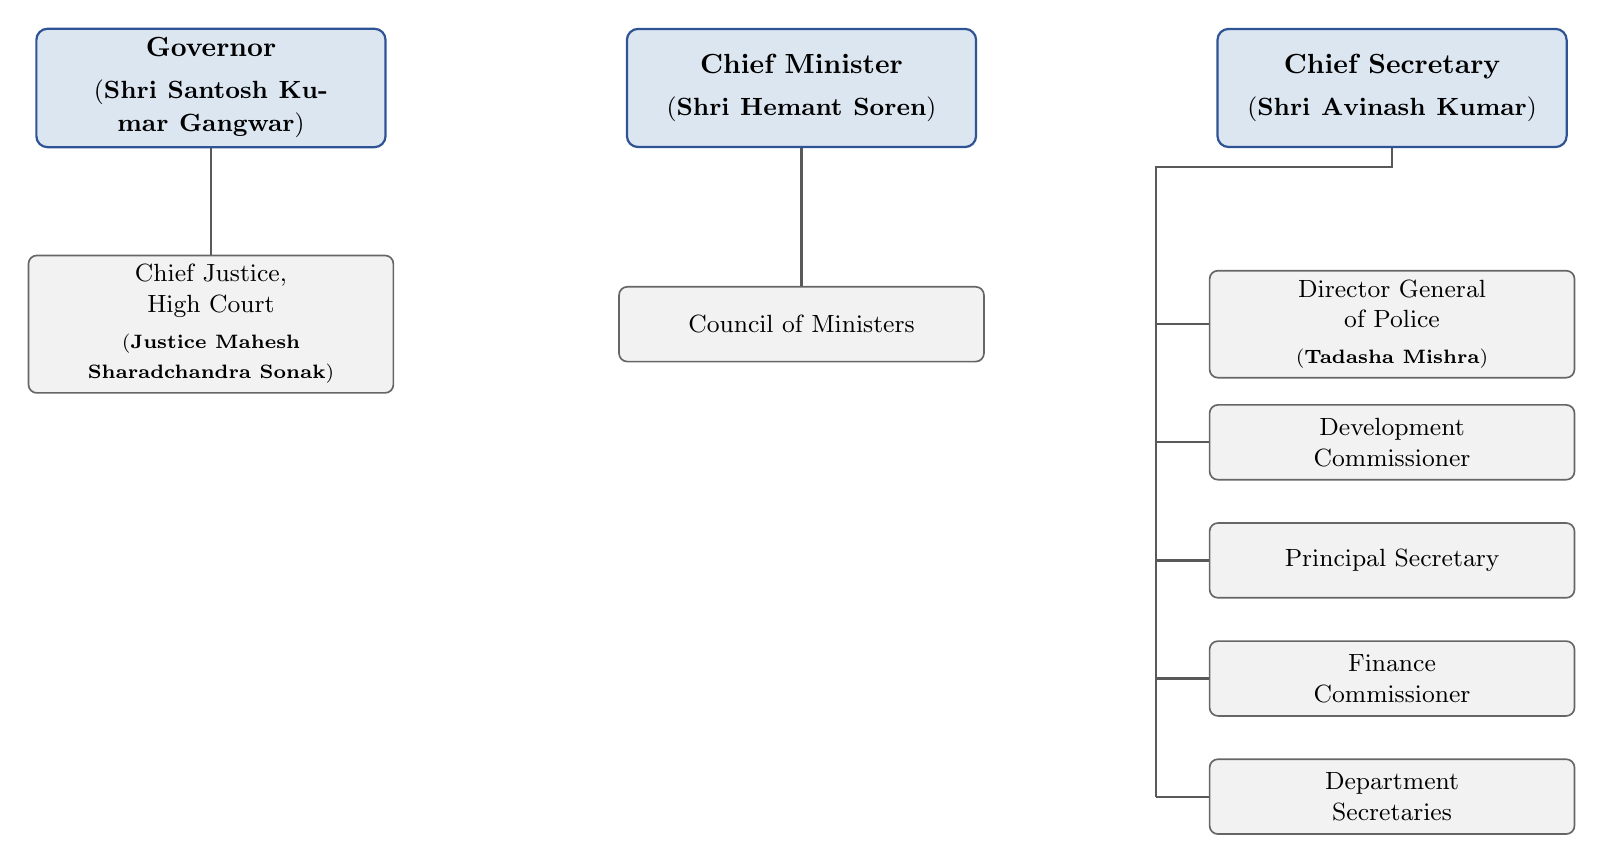
\begin{tikzpicture}[
  apex/.style={draw=apexline, fill=apexfill, rounded corners=4pt,
               line width=0.8pt, text width=4.2cm, align=center,
               minimum height=1.5cm, font=\bfseries},
  sub/.style={draw=subline, fill=subfill, rounded corners=3pt,
              line width=0.6pt, text width=4.4cm, align=center,
              minimum height=0.95cm, font=\small},
  link/.style={draw=black!65, line width=0.8pt}
]

% ---- apex level -----------------------------------------------------------
\node[apex] (gov) at (-7.5,0)
  {Governor\\[3pt]{\normalfont\small (\textbf{Shri Santosh Kumar Gangwar})}};

\node[apex] (cm) at (0,0)
  {Chief Minister\\[3pt]{\normalfont\small (\textbf{Shri Hemant Soren})}};

\node[apex] (cs) at (7.5,0)
  {Chief Secretary\\[3pt]{\normalfont\small (\textbf{Shri Avinash Kumar})}};

% ---- second level ---------------------------------------------------------
\node[sub] (cj) at (-7.5,-3.0)
  {Chief Justice,\\High Court\\[2pt]{\scriptsize (\textbf{Justice Mahesh Sharadchandra Sonak})}};

\node[sub] (com) at (0,-3.0)
  {Council of Ministers};

\node[sub] (dgp) at (7.5,-3.0)
  {Director General\\of Police\\[2pt]{\scriptsize (\textbf{Tadasha Mishra})}};

\node[sub] (dc) at (7.5,-4.50) {Development\\Commissioner};
\node[sub] (ps) at (7.5,-6.00) {Principal Secretary};
\node[sub] (fc) at (7.5,-7.50) {Finance\\Commissioner};
\node[sub] (ds) at (7.5,-9.00) {Department\\Secretaries};

% ---- links ----------------------------------------------------------------
\draw[link] (gov.south) -- (cj.north);
\draw[link] (cm.south)  -- (com.north);

\coordinate (busTop) at (4.5,-1.0);
\coordinate (busBot) at (4.5,-9.00);
\draw[link] (cs.south) -- (7.5,-1.0) -- (busTop) -- (busBot);
\foreach \n/\y in {dgp/-3.0, dc/-4.50, ps/-6.00, fc/-7.50, ds/-9.00}
  \draw[link] (4.5,\y) -- (\n.west);

\end{tikzpicture}%
}
\end{center}

\section*{How These Apex Level Inter-related}

\noindent{\footnotesize
\renewcommand{\arraystretch}{1.32}%
\begin{tabularx}{\textwidth}{@{}>{\raggedright\arraybackslash}p{3.5cm} X >{\raggedright\arraybackslash}p{3.2cm}@{}}
\toprule
\textbf{Pair} & \textbf{Nature of relation} & \textbf{Basis} \\
\midrule
Governor $\leftrightarrow$ Chief Minister &
Governor appoints the CM; ministers are appointed on the CM's advice; Governor acts on the aid and advice of the Council of Ministers; CM is the channel of communication and keeps the Governor informed. &
Arts.\ 163, 164, 167 \\
\addlinespace[4pt]
Governor $\leftrightarrow$ Chief Minister (discretion) &
May reserve a Bill, recommend President's Rule, or exercise discretion in a hung Assembly. &
Arts.\ 200, 356 \\
\addlinespace[4pt]
Chief Minister $\rightarrow$ Chief Secretary &
CM/Cabinet directs policy; CS is principal adviser, Secretary to the Cabinet, and head of the IAS bureaucracy; appointed by the Cabinet Appointment Committee. &
Non-constitutional \\
\addlinespace[4pt]
Governor $\leftrightarrow$ Chief Secretary &
Liaison, protocol and briefing only; no command---the CS answers to the elected government. &
Administrative practice \\
\addlinespace[4pt]
Chief Secretary $\rightarrow$ Department Secretaries &
Converts Cabinet decisions into implementation; supervises departmental secretaries and field administration. &
Service rules and executive instructions \\
\bottomrule
\end{tabularx}}


\noindent\textbf{Flow of authority:} Governor (appoints, advises) $\leftrightarrow$ Chief Minister (directs) $\rightarrow$ Chief Secretary (implements) $\rightarrow$ Department Secretaries $\rightarrow$ field administration.

\noindent\textbf{Accountability:} CM to the Assembly; CS to the CM/Cabinet; Governor to the President.

% ================================================================ Governor
\newpage
\section*{Hierarchies under the Governor}

\begin{center}
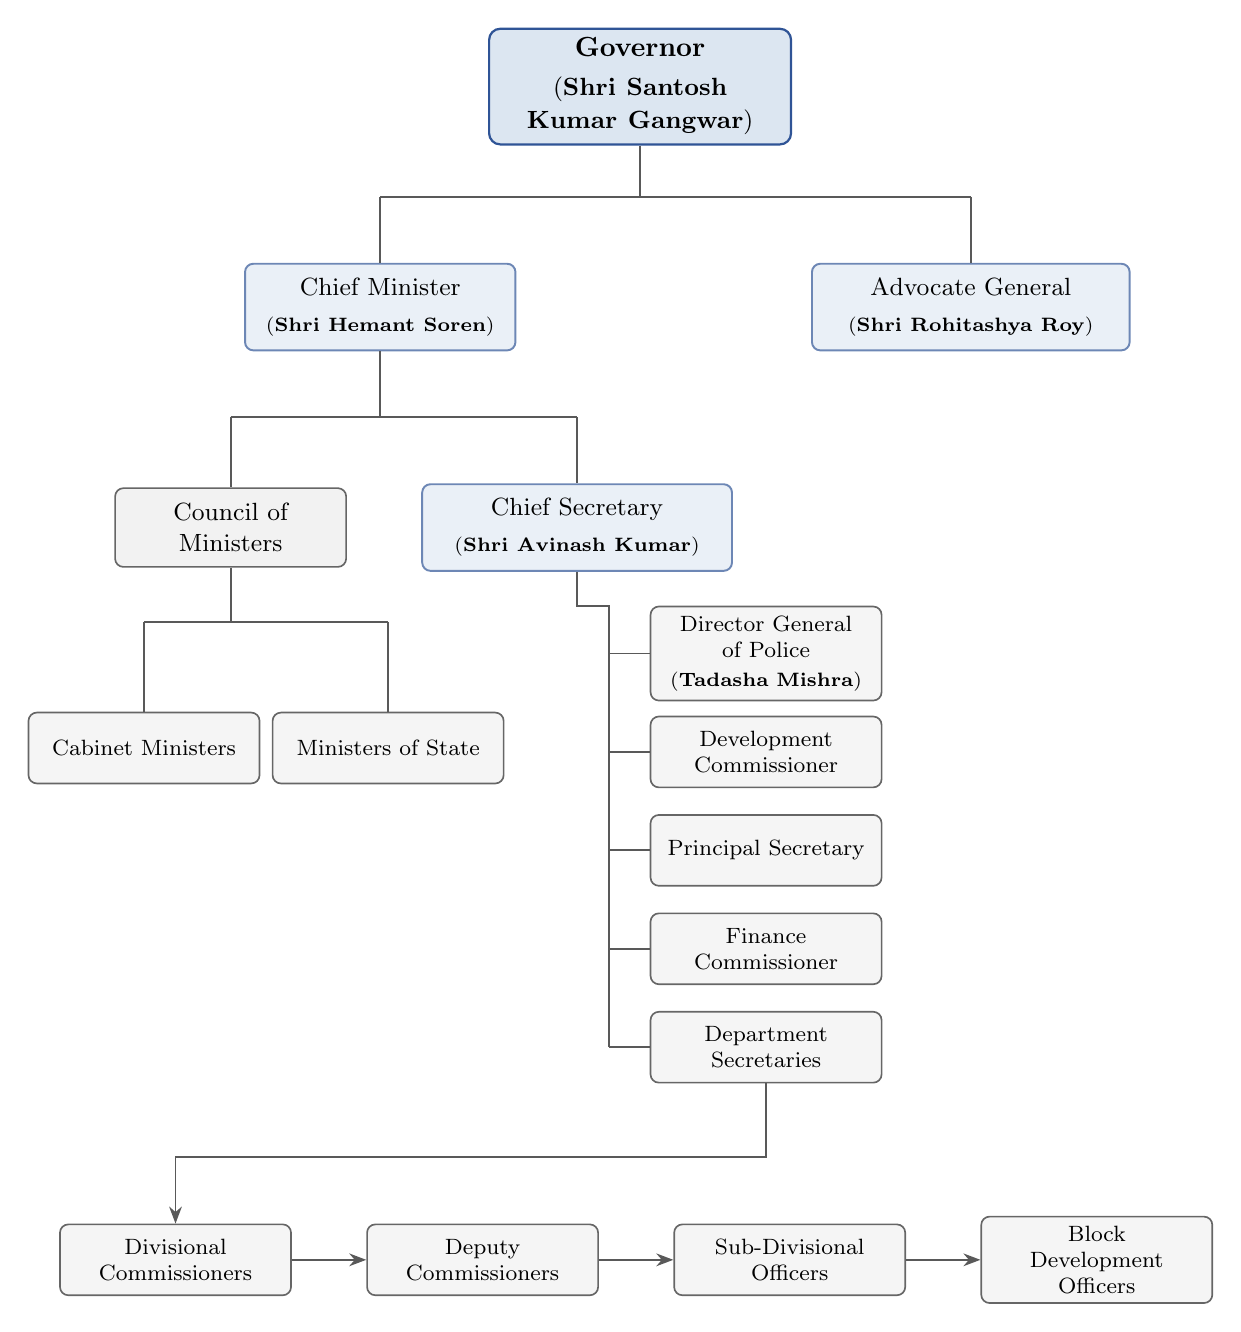
\begin{tikzpicture}
  \node[hroot] (gov) at (0,0)
    {Governor\\[2pt]{\normalfont\small (\textbf{Shri Santosh Kumar Gangwar})}};
  \node[hlvl] (cm) at (-3.3,-2.8)
    {Chief Minister\\[2pt]{\normalfont\scriptsize (\textbf{Shri Hemant Soren})}};
  \node[hlvl, text width=3.8cm] (ag) at (4.2,-2.8)
    {Advocate General\\[2pt]{\normalfont\scriptsize (\textbf{Shri Rohitashya Roy})}};

  \node[hsub] (council) at (-5.2,-5.6) {Council of Ministers};
  \node[hlvl, text width=3.7cm] (cs) at (-0.8,-5.6)
    {Chief Secretary\\[2pt]{\normalfont\scriptsize (\textbf{Shri Avinash Kumar})}};

  \node[hleaf] (cab) at (-6.3,-8.4) {Cabinet Ministers};
  \node[hleaf] (mos) at (-3.2,-8.4) {Ministers of State};

  \node[hleaf] (dgp) at (1.6,-7.2)
    {Director General\\of Police\\[1pt]{\scriptsize (\textbf{Tadasha Mishra})}};
  \node[hleaf] (dev) at (1.6,-8.45) {Development\\Commissioner};
  \node[hleaf] (ps)  at (1.6,-9.7)  {Principal Secretary};
  \node[hleaf] (fc)  at (1.6,-10.95) {Finance\\Commissioner};
  \node[hleaf] (ds)  at (1.6,-12.2) {Department\\Secretaries};

  \node[hleaf] (fdiv) at (-5.9,-14.9) {Divisional\\Commissioners};
  \node[hleaf] (fdc)  at (-2.0,-14.9) {Deputy\\Commissioners};
  \node[hleaf] (fsdo) at (1.9,-14.9)  {Sub-Divisional\\Officers};
  \node[hleaf] (fbdo) at (5.8,-14.9)  {Block\\Development\\Officers};

  \draw[hlink] (gov.south) -- (0,-1.4);
  \draw[hlink] (-3.3,-1.4) -- (4.2,-1.4);
  \draw[hlink] (-3.3,-1.4) -- (cm.north);
  \draw[hlink] (4.2,-1.4) -- (ag.north);

  \draw[hlink] (cm.south) -- (-3.3,-4.2);
  \draw[hlink] (-5.2,-4.2) -- (-0.8,-4.2);
  \draw[hlink] (-5.2,-4.2) -- (council.north);
  \draw[hlink] (-0.8,-4.2) -- (cs.north);

  \draw[hlink] (council.south) -- (-5.2,-6.8);
  \draw[hlink] (-6.3,-6.8) -- (-3.2,-6.8);
  \draw[hlink] (-6.3,-6.8) -- (cab.north);
  \draw[hlink] (-3.2,-6.8) -- (mos.north);

  \draw[hlink] (cs.south) -- (-0.8,-6.6) -- (-0.4,-6.6) -- (-0.4,-12.2);
  \draw[hlink] (-0.4,-7.2)   -- (dgp.west);
  \draw[hlink] (-0.4,-8.45)  -- (dev.west);
  \draw[hlink] (-0.4,-9.7)   -- (ps.west);
  \draw[hlink] (-0.4,-10.95) -- (fc.west);
  \draw[hlink] (-0.4,-12.2)  -- (ds.west);

  \draw[hlink, -{Stealth}] (ds.south) -- (1.6,-13.6) -- (-5.9,-13.6) -- (fdiv.north);
  \draw[hlink, -{Stealth}] (fdiv.east) -- (fdc.west);
  \draw[hlink, -{Stealth}] (fdc.east) -- (fsdo.west);
  \draw[hlink, -{Stealth}] (fsdo.east) -- (fbdo.west);
\end{tikzpicture}
\end{center}

\section*{Nature of the Blue Boxes}

\noindent{\scriptsize
\renewcommand{\arraystretch}{1.12}%
\begin{tabularx}{\textwidth}{@{}>{\raggedright\arraybackslash}p{2.6cm} >{\raggedright\arraybackslash}p{6.5cm} >{\raggedright\arraybackslash}X@{}}
\toprule
\textbf{Box} & \textbf{Nature of the office} & \textbf{Core mandate} \\
\midrule
Governor & Constitutional head of the State; appointed by the President; not a member of the legislature. & Appointments, assent to legislation, Chancellorship of universities and the discretionary powers listed above. \\
\addlinespace[2pt]
Chief Minister & Political head of the government; leader of the majority in the Assembly. & Formation of the ministry, policy and fiscal direction, and answerability to the Assembly. \\
\addlinespace[2pt]
Advocate General & Constitutional law officer (Art.~165); appointed by the Governor; not a minister. & Legal advice to the government, conduct of State litigation and audience in all State courts. \\
\addlinespace[2pt]
Chief Secretary & Non-constitutional administrative head; senior-most IAS officer; Secretary to the Cabinet. & Coordination of departments, monitoring of implementation and the cabinet secretariat. \\
\bottomrule
\end{tabularx}}

% ======================================================= Deputy Commissioner
\newpage
\section*{Functions of the Deputy Commissioner}

\begin{center}
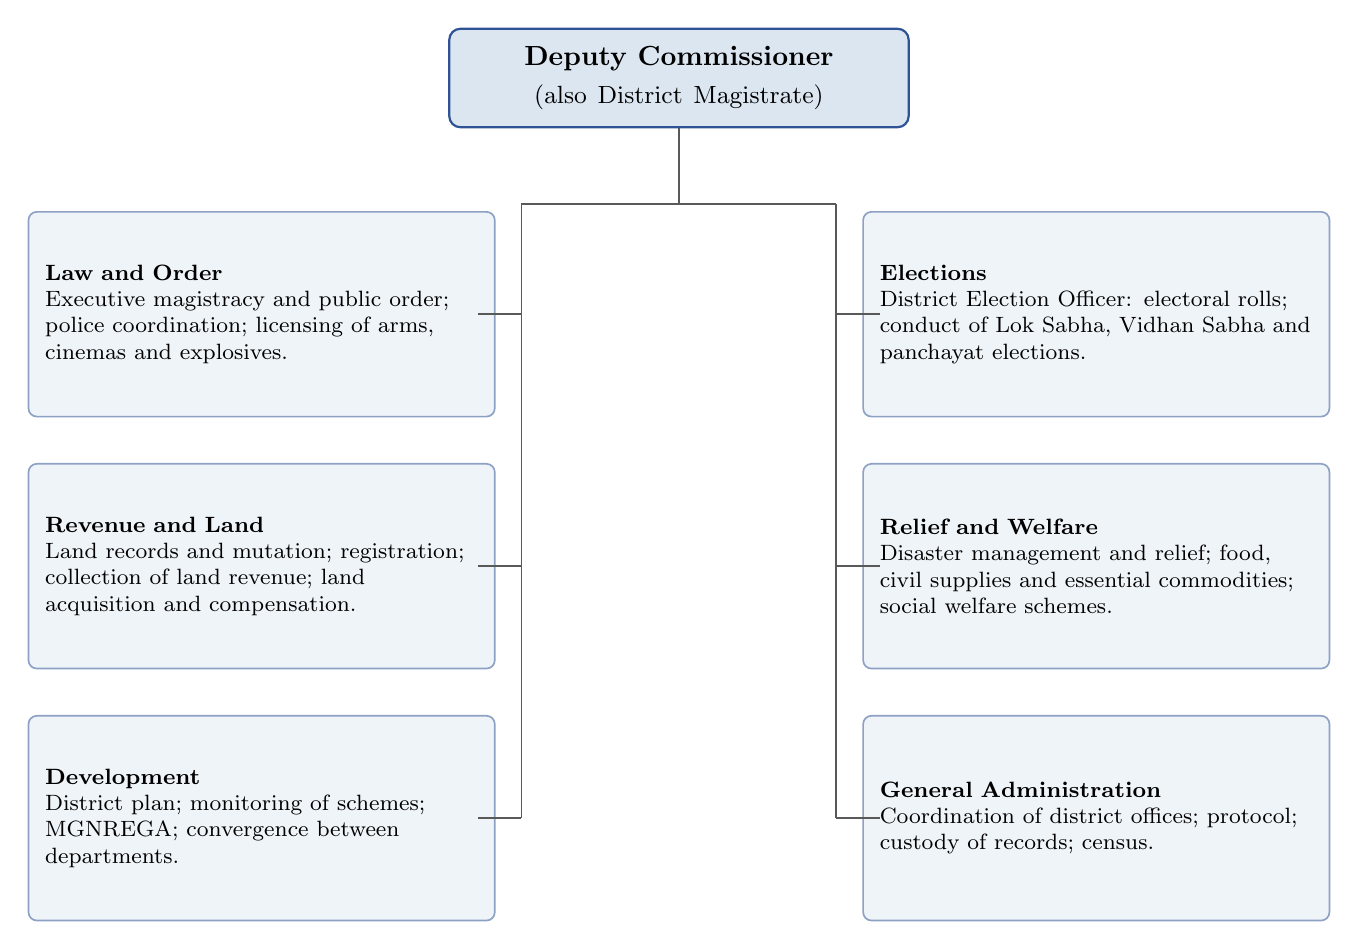
\begin{tikzpicture}
  \node[hroot, text width=5.6cm] (dc) at (0,0)
    {Deputy Commissioner\\[2pt]{\normalfont\small (also District Magistrate)}};

  \node[fnbox] (lo) at (-5.3,-3.0)
    {\textbf{Law and Order}\\ Executive magistracy and public order; police coordination; licensing of arms, cinemas and explosives.};
  \node[fnbox] (rev) at (-5.3,-6.2)
    {\textbf{Revenue and Land}\\ Land records and mutation; registration; collection of land revenue; land acquisition and compensation.};
  \node[fnbox] (dev) at (-5.3,-9.4)
    {\textbf{Development}\\ District plan; monitoring of schemes; MGNREGA; convergence between departments.};

  \node[fnbox] (elec) at (5.3,-3.0)
    {\textbf{Elections}\\ District Election Officer: electoral rolls; conduct of Lok Sabha, Vidhan Sabha and panchayat elections.};
  \node[fnbox] (rel) at (5.3,-6.2)
    {\textbf{Relief and Welfare}\\ Disaster management and relief; food, civil supplies and essential commodities; social welfare schemes.};
  \node[fnbox] (adm) at (5.3,-9.4)
    {\textbf{General Administration}\\ Coordination of district offices; protocol; custody of records; census.};

  \draw[hlink] (dc.south) -- (0,-1.6);
  \draw[hlink] (-2.0,-1.6) -- (2.0,-1.6);
  \draw[hlink] (-2.0,-1.6) -- (-2.0,-9.4);
  \draw[hlink] (2.0,-1.6) -- (2.0,-9.4);
  \foreach \y in {-3.0,-6.2,-9.4}{%
    \draw[hlink] (-2.0,\y) -- (-2.55,\y);%
    \draw[hlink] (2.0,\y) -- (2.55,\y);%
  }
\end{tikzpicture}
\end{center}

\vspace{2pt}
\noindent{\footnotesize\textbf{One officer, several roles.} The Deputy Commissioner is also District Magistrate (law and order), Collector (revenue) and District Election Officer (elections) --- one post wearing three hats, not three separate offices.}

% ======================================================= Ranchi worked example
\newpage
\section*{A Worked Example: Ranchi District to a \mbox{Village Panchayat}}

\begin{center}
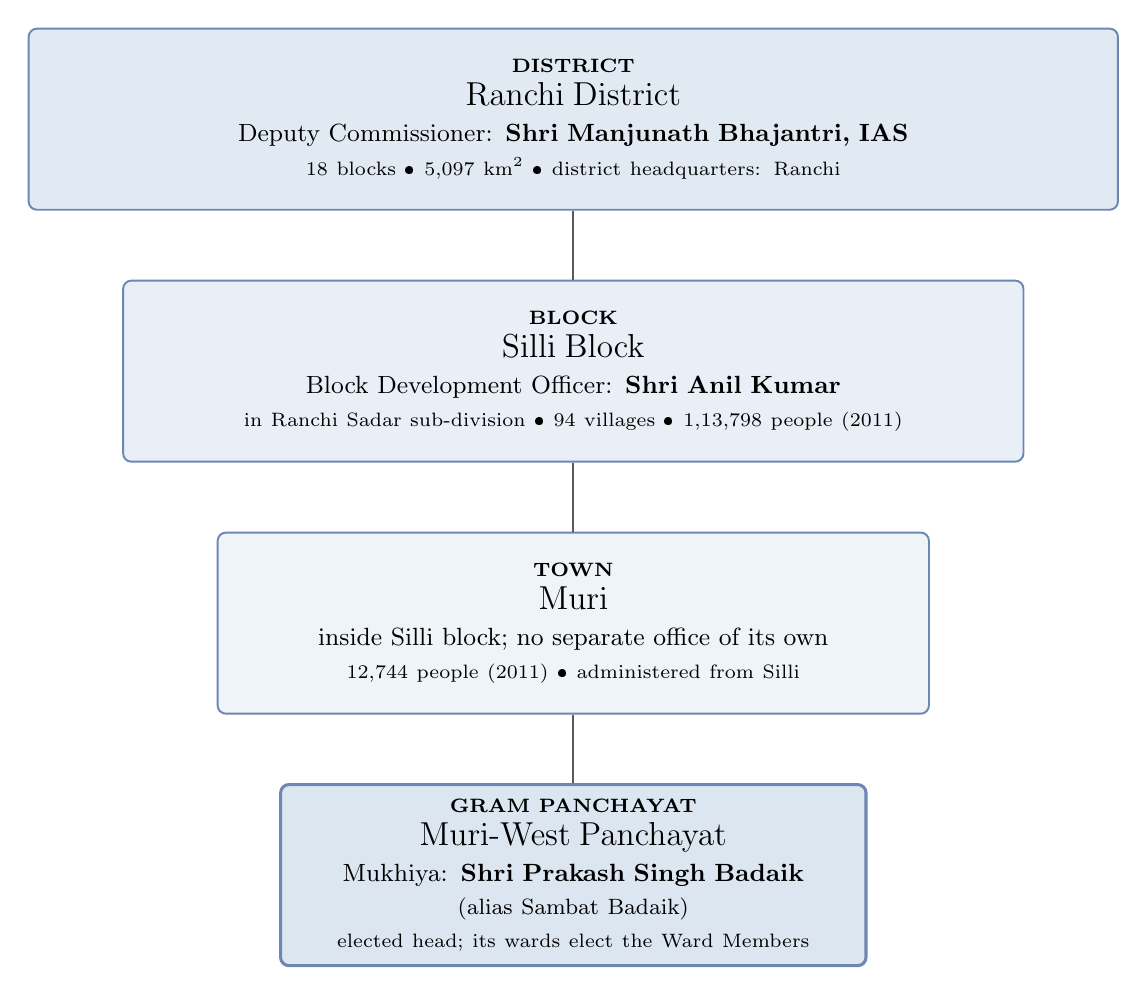
\begin{tikzpicture}
  \node[elecbox, text width=13.6cm, minimum height=2.3cm, fill=apexfill!85] (dist) at (0,0)
    {{\scriptsize\textbf{DISTRICT}}\\[1pt]
     {\large Ranchi District}\\[2pt]
     {Deputy Commissioner: \textbf{Shri Manjunath Bhajantri, IAS}}\\[1pt]
     {\scriptsize 18 blocks \textbullet\ 5,097 km\textsuperscript{2} \textbullet\ district headquarters: Ranchi}};

  \node[elecbox, text width=11.2cm, minimum height=2.3cm, fill=apexfill!65] (blk) at (0,-3.2)
    {{\scriptsize\textbf{BLOCK}}\\[1pt]
     {\large Silli Block}\\[2pt]
     {Block Development Officer: \textbf{Shri Anil Kumar}}\\[1pt]
     {\scriptsize in Ranchi Sadar sub-division \textbullet\ 94 villages \textbullet\ 1,13,798 people (2011)}};

  \node[elecbox, text width=8.8cm, minimum height=2.3cm, fill=apexfill!45] (muri) at (0,-6.4)
    {{\scriptsize\textbf{TOWN}}\\[1pt]
     {\large Muri}\\[2pt]
     {inside Silli block; no separate office of its own}\\[1pt]
     {\scriptsize 12,744 people (2011) \textbullet\ administered from Silli}};

  \node[elecbox, text width=7.2cm, minimum height=2.3cm, fill=apexfill, line width=1.1pt] (gp) at (0,-9.6)
    {{\scriptsize\textbf{GRAM PANCHAYAT}}\\[1pt]
     {\large Muri-West Panchayat}\\[2pt]
     {Mukhiya: \textbf{Shri Prakash Singh Badaik}\\[1pt]
      {\footnotesize (alias Sambat Badaik)}}\\[1pt]
     {\scriptsize elected head; its wards elect the Ward Members}};

  \draw[hlink] (dist.south) -- (blk.north);
  \draw[hlink] (blk.south) -- (muri.north);
  \draw[hlink] (muri.south) -- (gp.north);
\end{tikzpicture}
\end{center}

\vspace{2pt}
\noindent{\footnotesize\textbf{Reading the example.} Silli is a \emph{block}, not a sub-division, and Muri is a town inside Silli block --- so the chain runs District $\rightarrow$ Block $\rightarrow$ Gram Panchayat, with Muri marking the locality, not a separate tier. The Deputy Commissioner's name is as of 2026; the BDO and the Mukhiya are as per the latest district records available (2024--25).}

% ======================================================= Ranchi police example
\newpage
\section*{A Worked Example: Ranchi Police from the Range to Muri Thana}

\begin{center}
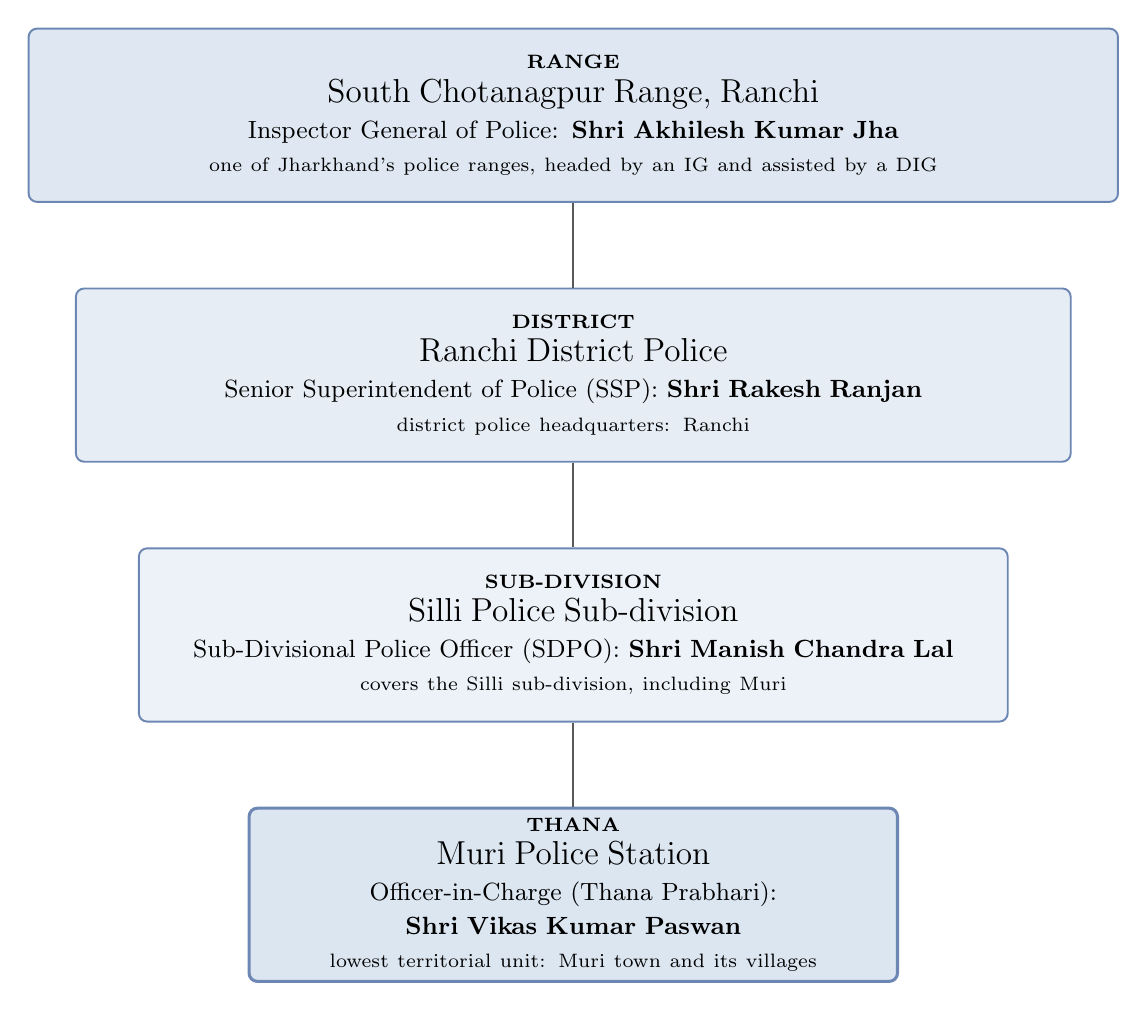
\begin{tikzpicture}
  \node[elecbox, text width=13.6cm, minimum height=2.2cm, fill=apexfill!90] (range) at (0,0)
    {{\scriptsize\textbf{RANGE}}\\[1pt]
     {\large South Chotanagpur Range, Ranchi}\\[2pt]
     {Inspector General of Police: \textbf{Shri Akhilesh Kumar Jha}}\\[1pt]
     {\scriptsize one of Jharkhand's police ranges, headed by an IG and assisted by a DIG}};

  \node[elecbox, text width=12.4cm, minimum height=2.2cm, fill=apexfill!70] (ssp) at (0,-3.3)
    {{\scriptsize\textbf{DISTRICT}}\\[1pt]
     {\large Ranchi District Police}\\[2pt]
     {Senior Superintendent of Police (SSP): \textbf{Shri Rakesh Ranjan}}\\[1pt]
     {\scriptsize district police headquarters: Ranchi}};

  \node[elecbox, text width=10.8cm, minimum height=2.2cm, fill=apexfill!50] (sdpo) at (0,-6.6)
    {{\scriptsize\textbf{SUB-DIVISION}}\\[1pt]
     {\large Silli Police Sub-division}\\[2pt]
     {Sub-Divisional Police Officer (SDPO): \textbf{Shri Manish Chandra Lal}}\\[1pt]
     {\scriptsize covers the Silli sub-division, including Muri}};

  \node[elecbox, text width=8.0cm, minimum height=2.2cm, fill=apexfill, line width=1.1pt] (thana) at (0,-9.9)
    {{\scriptsize\textbf{THANA}}\\[1pt]
     {\large Muri Police Station}\\[2pt]
     {Officer-in-Charge (Thana Prabhari):\\[1pt]
      \textbf{Shri Vikas Kumar Paswan}}\\[1pt]
     {\scriptsize lowest territorial unit: Muri town and its villages}};

  \draw[hlink] (range.south) -- (ssp.north);
  \draw[hlink] (ssp.south) -- (sdpo.north);
  \draw[hlink] (sdpo.south) -- (thana.north);
\end{tikzpicture}
\end{center}

\vspace{2pt}
\noindent{\footnotesize\textbf{Reading the example.} The IG heads the range, the SSP the district, the SDPO a police sub-division and the thana in-charge the police station --- the lowest territorial unit of policing. Above the range sits the Director General of Police, Jharkhand. Names are as of 2026; the SDPO and the thana in-charge took their posts in the May 2026 reshuffle.}

% ======================================================= Muri sector page
\newpage
\section*{Muri at a Glance: Sector by Sector}

\begin{center}
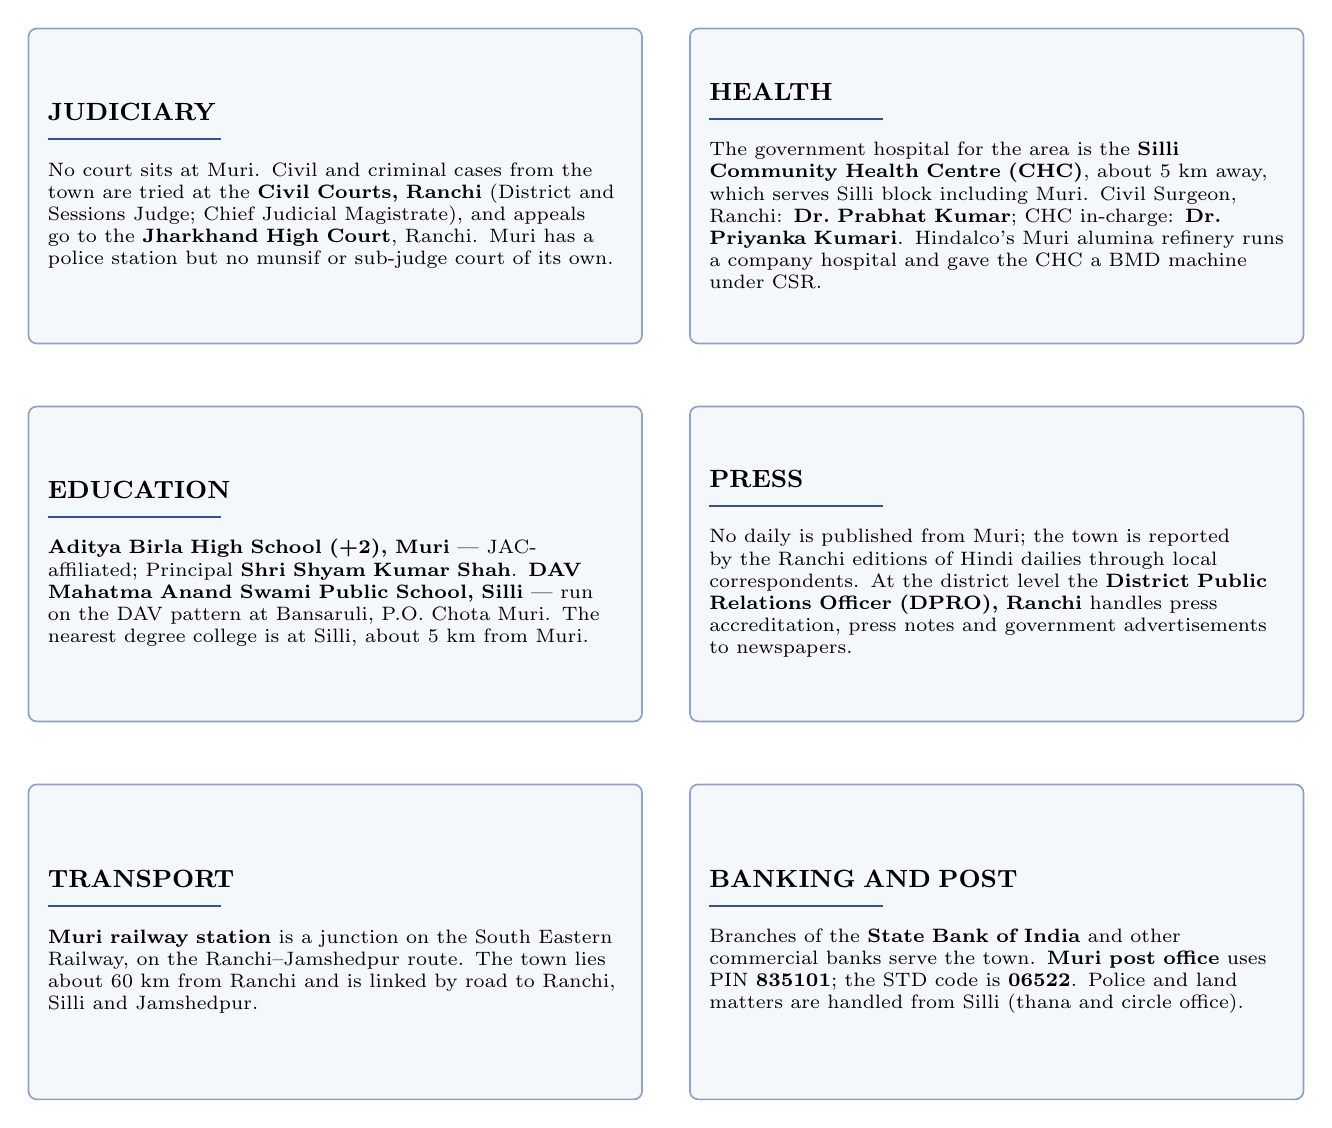
\begin{tikzpicture}
  \node[secbox] at (-4.2,-0.2)
    {{\textbf{\small JUDICIARY}}\\[-1pt]{\color{apexline}\rule{2.2cm}{0.7pt}}\\[5pt]
     No court sits at Muri. Civil and criminal cases from the town are tried at the
     \textbf{Civil Courts, Ranchi} (District and Sessions Judge; Chief Judicial Magistrate),
     and appeals go to the \textbf{Jharkhand High Court}, Ranchi. Muri has a police station
     but no munsif or sub-judge court of its own.};

  \node[secbox] at (4.2,-0.2)
    {{\textbf{\small HEALTH}}\\[-1pt]{\color{apexline}\rule{2.2cm}{0.7pt}}\\[5pt]
     The government hospital for the area is the \textbf{Silli Community Health Centre (CHC)},
     about 5 km away, which serves Silli block including Muri. Civil Surgeon, Ranchi:
     \textbf{Dr.\ Prabhat Kumar}; CHC in-charge: \textbf{Dr.\ Priyanka Kumari}. Hindalco's
     Muri alumina refinery runs a company hospital and gave the CHC a BMD machine under CSR.};

  \node[secbox] at (-4.2,-5.0)
    {{\textbf{\small EDUCATION}}\\[-1pt]{\color{apexline}\rule{2.2cm}{0.7pt}}\\[5pt]
     \textbf{Aditya Birla High School (+2), Muri} --- JAC-affiliated; Principal
     \textbf{Shri Shyam Kumar Shah}. \textbf{DAV Mahatma Anand Swami Public School, Silli}
     --- run on the DAV pattern at Bansaruli, P.O.\ Chota Muri. The nearest degree college
     is at Silli, about 5 km from Muri.};

  \node[secbox] at (4.2,-5.0)
    {{\textbf{\small PRESS}}\\[-1pt]{\color{apexline}\rule{2.2cm}{0.7pt}}\\[5pt]
     No daily is published from Muri; the town is reported by the Ranchi editions of Hindi
     dailies through local correspondents. At the district level the \textbf{District Public
     Relations Officer (DPRO), Ranchi} handles press accreditation, press notes and
     government advertisements to newspapers.};

  \node[secbox] at (-4.2,-9.8)
    {{\textbf{\small TRANSPORT}}\\[-1pt]{\color{apexline}\rule{2.2cm}{0.7pt}}\\[5pt]
     \textbf{Muri railway station} is a junction on the South Eastern Railway, on the
     Ranchi--Jamshedpur route. The town lies about 60 km from Ranchi and is linked by road
     to Ranchi, Silli and Jamshedpur.};

  \node[secbox] at (4.2,-9.8)
    {{\textbf{\small BANKING AND POST}}\\[-1pt]{\color{apexline}\rule{2.2cm}{0.7pt}}\\[5pt]
     Branches of the \textbf{State Bank of India} and other commercial banks serve the town.
     \textbf{Muri post office} uses PIN \textbf{835101}; the STD code is \textbf{06522}.
     Police and land matters are handled from Silli (thana and circle office).};
\end{tikzpicture}
\end{center}

\vspace{2pt}
\noindent{\footnotesize Sector details are as per the latest available district records and reports (2024--26); the police set-up is on the previous page.}

% ============================================================= Advocate General
\newpage
\section*{Office of the Advocate General}

\begin{center}
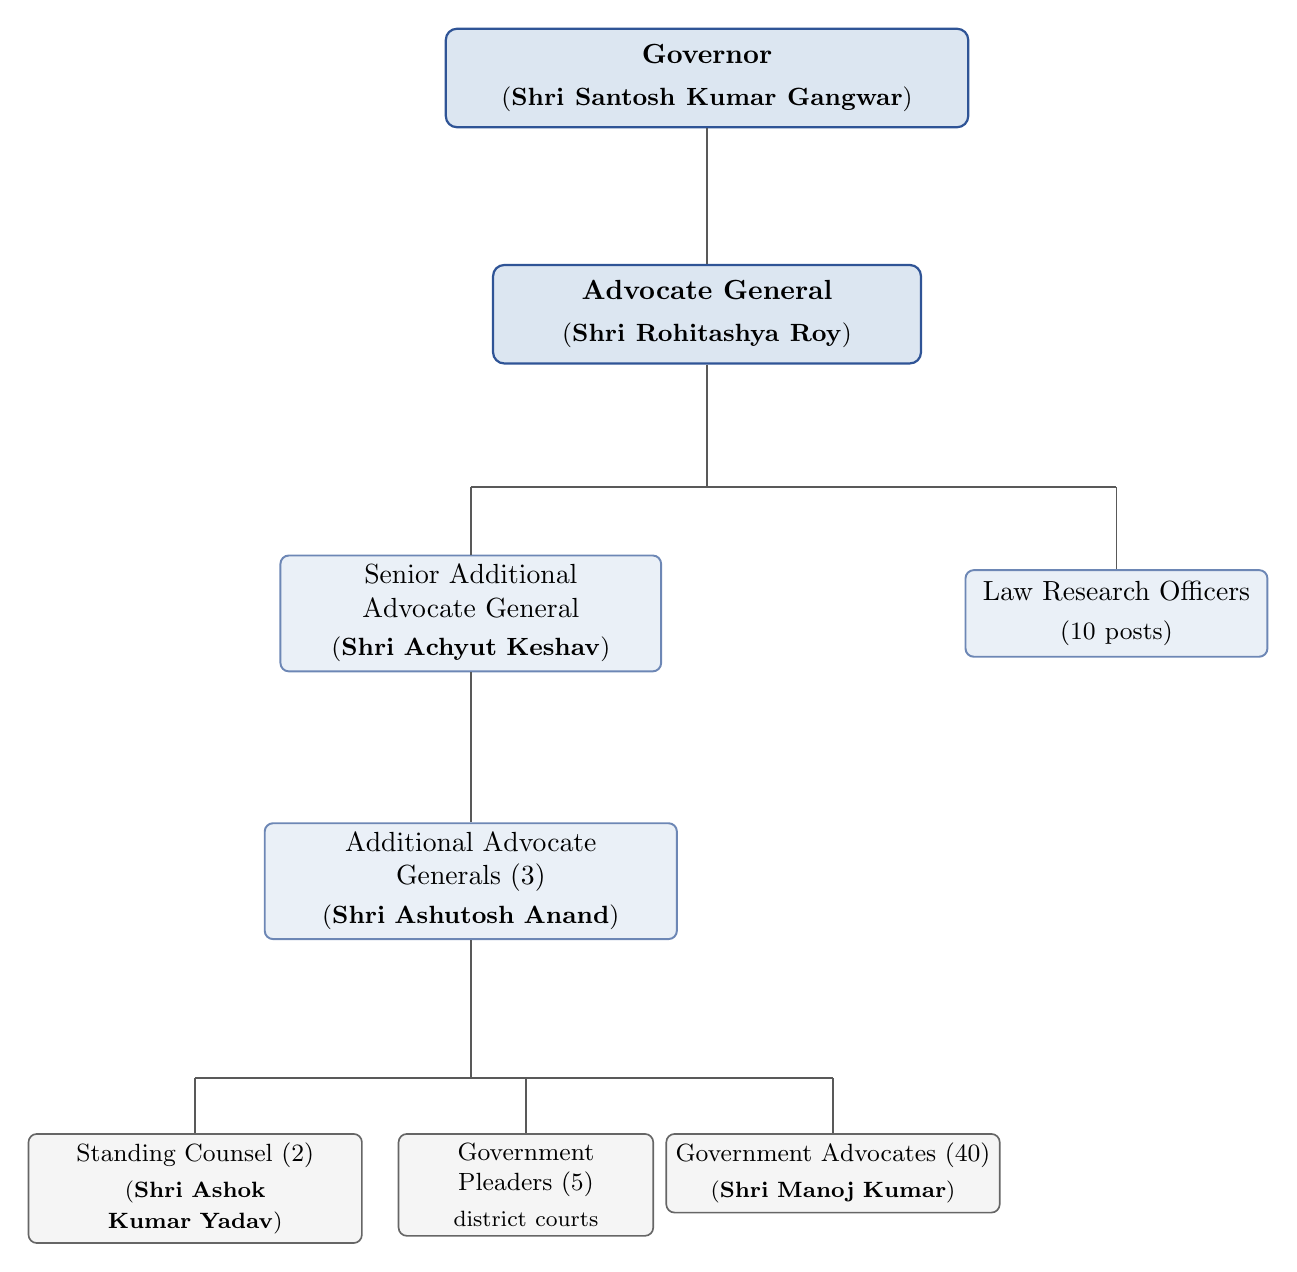
\begin{tikzpicture}
  \node[hroot, text width=6.4cm] (gov) at (0,0)
    {Governor\\[3pt]{\normalfont\small (\textbf{Shri Santosh Kumar Gangwar})}};

  \node[hroot, text width=5.2cm] (ag) at (0,-3.0)
    {Advocate General\\[3pt]{\normalfont\small (\textbf{Shri Rohitashya Roy})}};

  \node[hlvl, text width=4.6cm, font=\normalsize] (saag) at (-3.0,-6.8)
    {Senior Additional Advocate General\\[2pt]{\normalfont\small (\textbf{Shri Achyut Keshav})}};

  \node[hlvl, text width=3.6cm, font=\normalsize] (lro) at (5.2,-6.8)
    {Law Research Officers\\[2pt]{\normalfont\small (10 posts)}};

  \node[hlvl, text width=5.0cm, font=\normalsize] (aag) at (-3.0,-10.2)
    {Additional Advocate Generals (3)\\[2pt]{\normalfont\small (\textbf{Shri Ashutosh Anand})}};

  \node[hleaf, text width=4.0cm, font=\small, anchor=north] (sc) at (-6.5,-13.4)
    {Standing Counsel (2)\\[2pt]{\footnotesize (\textbf{Shri Ashok Kumar Yadav})}};

  \node[hleaf, text width=3.0cm, font=\small, anchor=north] (gp) at (-2.3,-13.4)
    {Government Pleaders (5)\\[2pt]{\footnotesize district courts}};

  \node[hleaf, text width=4.0cm, font=\small, anchor=north] (ga) at (1.6,-13.4)
    {Government Advocates (40)\\[2pt]{\footnotesize (\textbf{Shri Manoj Kumar})}};

  \draw[hlink] (gov.south) -- (ag.north);

  \draw[hlink] (ag.south) -- (0,-5.2);
  \draw[hlink] (-3.0,-5.2) -- (5.2,-5.2);
  \draw[hlink] (-3.0,-5.2) -- (saag.north);
  \draw[hlink] (5.2,-5.2) -- (lro.north);

  \draw[hlink] (saag.south) -- (aag.north);

  \draw[hlink] (aag.south) -- (-3.0,-12.7);
  \draw[hlink] (-6.5,-12.7) -- (1.6,-12.7);
  \draw[hlink] (-6.5,-12.7) -- (sc.north);
  \draw[hlink] (-2.3,-12.7) -- (gp.north);
  \draw[hlink] (1.6,-12.7) -- (ga.north);
\end{tikzpicture}
\end{center}

\noindent{\footnotesize Posts sanctioned in the Office of the Advocate General under the Jharkhand Law Officer (Engagement) Rules, 2026; names as of September 2026.}

% ============================================================= Council of Ministers
\newpage
\section*{Council of Ministers}

\begin{center}
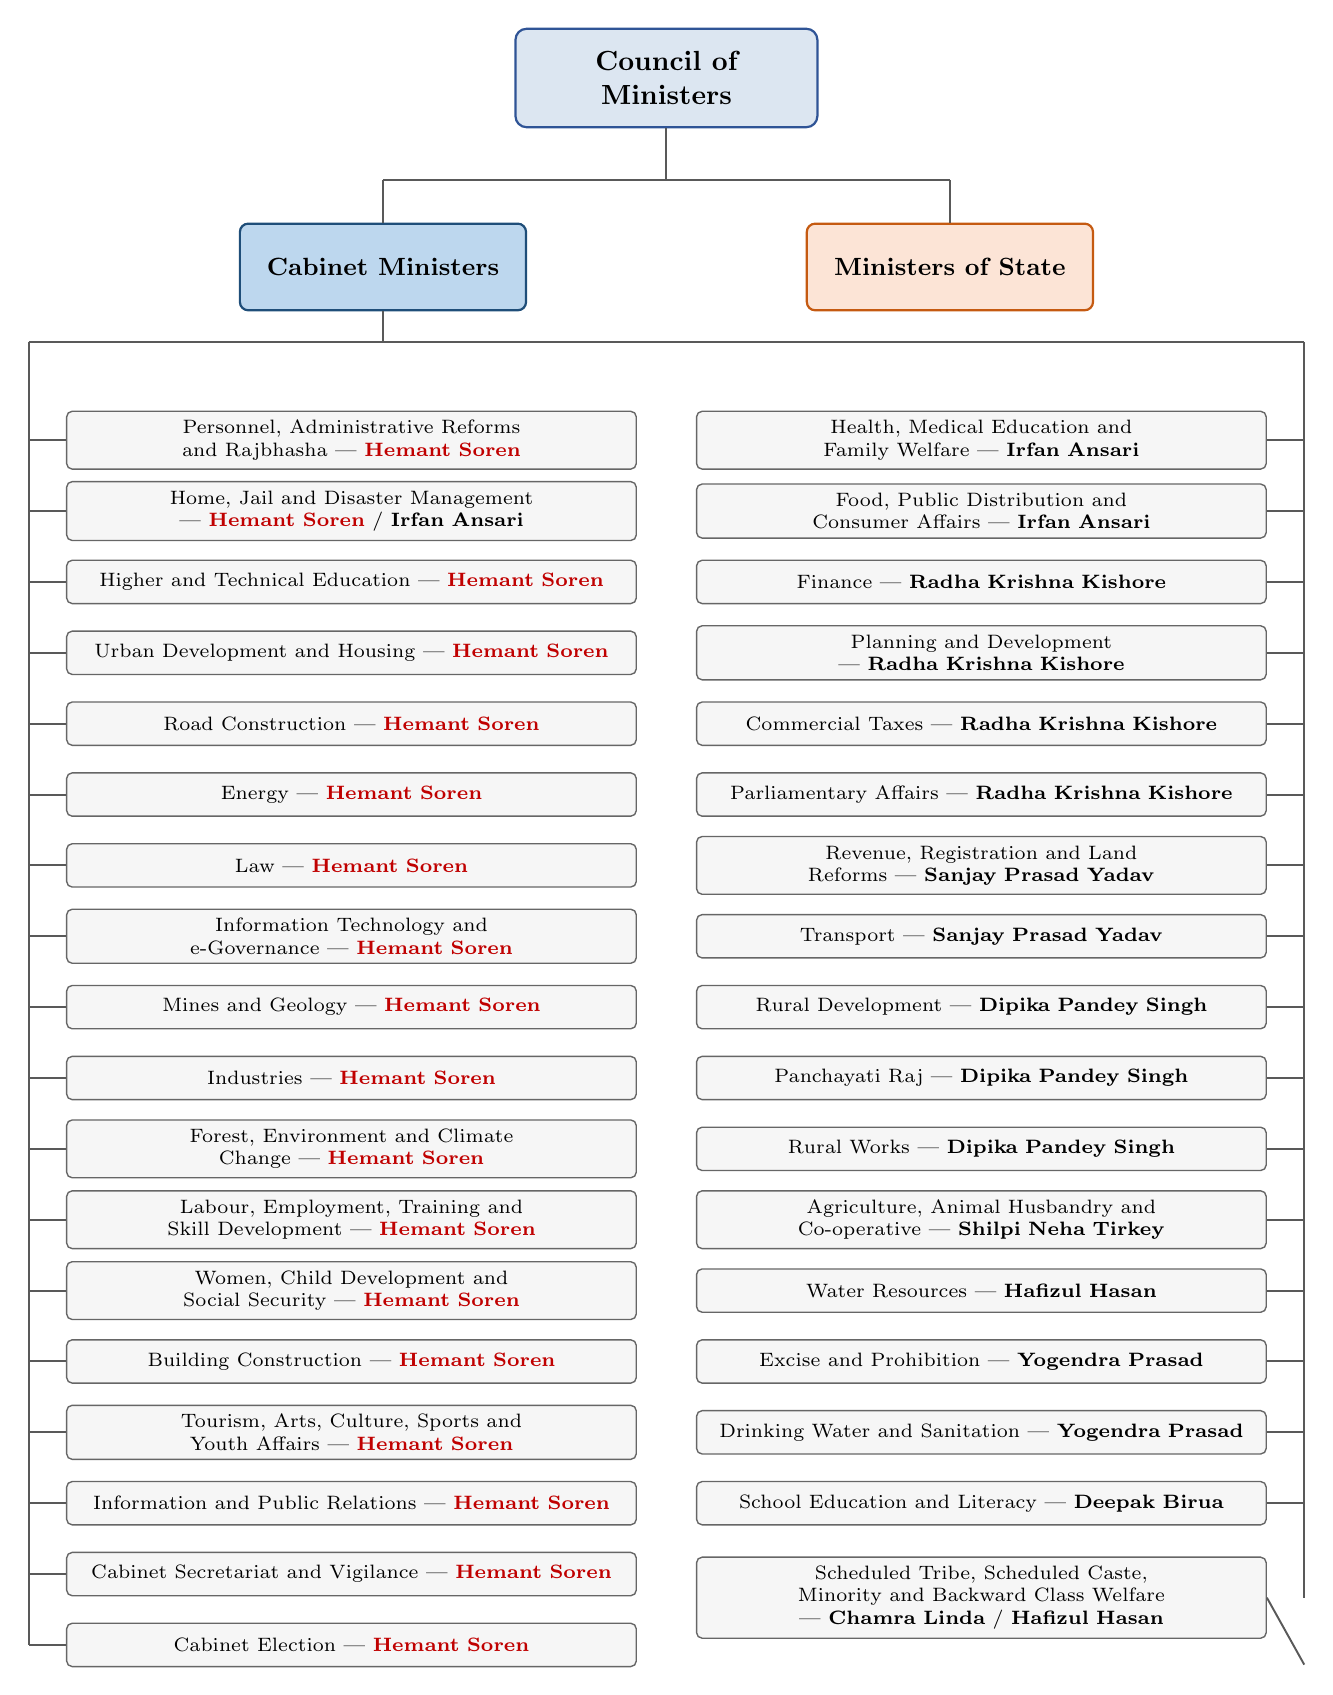
\begin{tikzpicture}
  \node[hroot] (com) at (0,0) {Council of Ministers};

  \node[cabbox] (cab) at (-3.6,-2.4) {Cabinet Ministers};
  \node[mosbox] (mos) at (3.6,-2.4) {Ministers of State};

  % \node[hsub, anchor=north, text width=5.4cm] (charge) at (3.6,-3.7)
  %   {Independent charge or attached\\to a Cabinet Minister};

  \draw[hlink] (com.south) -- (0,-1.3);
  \draw[hlink] (-3.6,-1.3) -- (3.6,-1.3);
  \draw[hlink] (-3.6,-1.3) -- (cab.north);
  \draw[hlink] (3.6,-1.3) -- (mos.north);
  % \draw[hlink] (mos.south) -- (charge.north);

  \draw[hlink] (cab.south) -- (-3.6,-3.35);
  \draw[hlink] (-8.1,-3.35) -- (8.1,-3.35);
  \draw[hlink] (-8.1,-3.35) -- (-8.1,-19.9);
  \draw[hlink] (8.1,-3.35) -- (8.1,-19.3);

  \foreach \nm [count=\i from 0] in {%
    {Personnel, Administrative Reforms and Rajbhasha --- \textbf{\textcolor{cmred}{Hemant Soren}}},%
    {Home, Jail and Disaster Management --- \textbf{\textcolor{cmred}{Hemant Soren}} / \textbf{Irfan Ansari}},%
    {Higher and Technical Education --- \textbf{\textcolor{cmred}{Hemant Soren}}},%
    {Urban Development and Housing --- \textbf{\textcolor{cmred}{Hemant Soren}}},%
    {Road Construction --- \textbf{\textcolor{cmred}{Hemant Soren}}},%
    {Energy --- \textbf{\textcolor{cmred}{Hemant Soren}}},%
    {Law --- \textbf{\textcolor{cmred}{Hemant Soren}}},%
    {Information Technology and \mbox{e-Governance} --- \textbf{\textcolor{cmred}{Hemant Soren}}},%
    {Mines and Geology --- \textbf{\textcolor{cmred}{Hemant Soren}}},%
    {Industries --- \textbf{\textcolor{cmred}{Hemant Soren}}},%
    {Forest, Environment and Climate Change --- \textbf{\textcolor{cmred}{Hemant Soren}}},%
    {Labour, Employment, Training and Skill Development --- \textbf{\textcolor{cmred}{Hemant Soren}}},%
    {Women, Child Development and Social Security --- \textbf{\textcolor{cmred}{Hemant Soren}}},%
    {Building Construction --- \textbf{\textcolor{cmred}{Hemant Soren}}},%
    {Tourism, Arts, Culture, Sports and Youth Affairs --- \textbf{\textcolor{cmred}{Hemant Soren}}},%
    {Information and Public Relations --- \textbf{\textcolor{cmred}{Hemant Soren}}},%
    {Cabinet Secretariat and Vigilance --- \textbf{\textcolor{cmred}{Hemant Soren}}},%
    {Cabinet Election --- \textbf{\textcolor{cmred}{Hemant Soren}}}%
  }{%
    \pgfmathsetmacro{\yy}{-4.6-0.9*\i}%
    \node[minbox, text width=7.0cm, minimum height=0.55cm] (a\i) at (-4.0,\yy) {\nm};%
    \draw[hlink] (-8.1,\yy) -- (a\i.west);%
  }

  \foreach \nm [count=\i from 0] in {%
    {Health, Medical Education and Family Welfare --- \textbf{Irfan Ansari}},%
    {Food, Public Distribution and Consumer Affairs --- \textbf{Irfan Ansari}},%
    {Finance --- \textbf{Radha Krishna Kishore}},%
    {Planning and Development --- \textbf{Radha Krishna Kishore}},%
    {Commercial Taxes --- \textbf{Radha Krishna Kishore}},%
    {Parliamentary Affairs --- \textbf{Radha Krishna Kishore}},%
    {Revenue, Registration and Land Reforms --- \textbf{Sanjay Prasad Yadav}},%
    {Transport --- \textbf{Sanjay Prasad Yadav}},%
    {Rural Development --- \textbf{Dipika Pandey Singh}},%
    {Panchayati Raj --- \textbf{Dipika Pandey Singh}},%
    {Rural Works --- \textbf{Dipika Pandey Singh}},%
    {Agriculture, Animal Husbandry and Co-operative --- \textbf{Shilpi Neha Tirkey}},%
    {Water Resources --- \textbf{Hafizul Hasan}},%
    {Excise and Prohibition --- \textbf{Yogendra Prasad}},%
    {Drinking Water and Sanitation --- \textbf{Yogendra Prasad}},%
    {School Education and Literacy --- \textbf{Deepak Birua}}%
  }{%
    \pgfmathsetmacro{\yy}{-4.6-0.9*\i}%
    \node[minbox, text width=7.0cm, minimum height=0.55cm] (b\i) at (4.0,\yy) {\nm};%
    \draw[hlink] (8.1,\yy) -- (b\i.east);%
  }

  \node[minbox, text width=7.0cm, minimum height=0.55cm] (bw) at (4.0,-19.3)
    {Scheduled Tribe, Scheduled Caste, Minority and Backward Class Welfare
     --- \textbf{Chamra Linda} / \textbf{Hafizul Hasan}};
  \draw[hlink] (8.1,-20.15) -- (bw.east);
\end{tikzpicture}
\end{center}

\noindent{\scriptsize Portfolios as of September 2026.\quad \textcolor{cmred}{\textbf{Red}} = held directly by the Chief Minister.}

\newpage
\section*{Cabinet Minister vs Minister of State}

\noindent{\footnotesize
\renewcommand{\arraystretch}{1.24}%
\begin{tabularx}{\textwidth}{@{}>{\raggedright\arraybackslash}p{2.8cm} >{\raggedright\arraybackslash}X >{\raggedright\arraybackslash}X@{}}
\toprule
 & \textbf{Cabinet Minister} & \textbf{Minister of State} \\
\midrule
Rank & Senior minister of Cabinet rank; heads a ministry and sits in the Cabinet. & Junior minister; assists a Cabinet Minister, or holds independent charge of a ministry. \\
\addlinespace[3pt]
Cabinet & Attends Cabinet meetings and shares in collective decisions. & Attends only if specially invited. \\
\addlinespace[3pt]
Work & Sets the ministry's policy, supervises its departments and answers for the whole ministry in the House. & Runs the allotted subjects, assists the Cabinet Minister and represents the ministry in the House. \\
\addlinespace[3pt]
Accountability & Collective responsibility (Art.~164(2)); answerable for the entire ministry. & Same collective responsibility; answerable for the allotted work. \\
\bottomrule
\end{tabularx}}

\vspace{4pt}
\noindent{\footnotesize Both are appointed by the Governor on the advice of the Chief Minister, and must be, or become within six months, members of either House.}

\vspace{6pt}
\noindent{\footnotesize\textbf{How they function.} The Cabinet Minister decides; the Minister of State executes the allotted part and carries the ministry's case in the House. Both work through the same departmental secretaries, and the Cabinet Minister remains answerable for the ministry as a whole.}

% ======================================================= Election hierarchy
\newpage
\section*{Election Hierarchy: From MLA to the Village}

\begin{center}
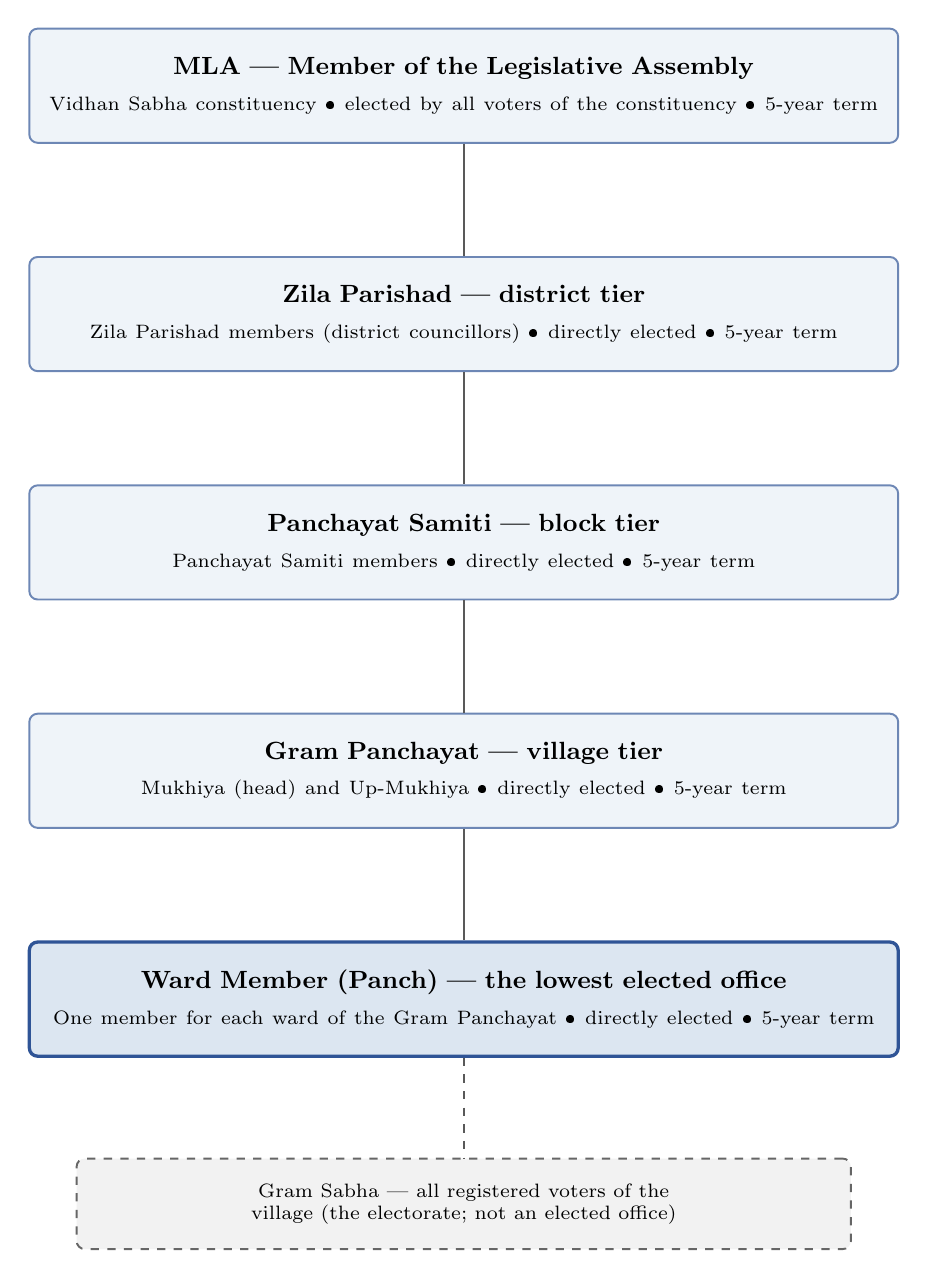
\begin{tikzpicture}
  \node[elecbox] (mla) at (0,0)
    {\textbf{MLA --- Member of the Legislative Assembly}\\[2pt]
     {\scriptsize Vidhan Sabha constituency \textbullet\ elected by all voters of the constituency \textbullet\ 5-year term}};
  \node[elecbox] (zp) at (0,-2.9)
    {\textbf{Zila Parishad --- district tier}\\[2pt]
     {\scriptsize Zila Parishad members (district councillors) \textbullet\ directly elected \textbullet\ 5-year term}};
  \node[elecbox] (psa) at (0,-5.8)
    {\textbf{Panchayat Samiti --- block tier}\\[2pt]
     {\scriptsize Panchayat Samiti members \textbullet\ directly elected \textbullet\ 5-year term}};
  \node[elecbox] (gp) at (0,-8.7)
    {\textbf{Gram Panchayat --- village tier}\\[2pt]
     {\scriptsize Mukhiya (head) and Up-Mukhiya \textbullet\ directly elected \textbullet\ 5-year term}};
  \node[elecbox, draw=apexline, line width=1.2pt, fill=apexfill] (ward) at (0,-11.6)
    {\textbf{Ward Member (Panch) --- the lowest elected office}\\[2pt]
     {\scriptsize One member for each ward of the Gram Panchayat \textbullet\ directly elected \textbullet\ 5-year term}};
  \node[elecbox, draw=subline, dashed, fill=subfill, font=\scriptsize,
        minimum height=1.15cm, text width=9.6cm] (gs) at (0,-14.2)
    {Gram Sabha --- all registered voters of the village (the electorate; not an elected office)};

  \draw[hlink] (mla.south) -- (zp.north);
  \draw[hlink] (zp.south) -- (psa.north);
  \draw[hlink] (psa.south) -- (gp.north);
  \draw[hlink] (gp.south) -- (ward.north);
  \draw[hlink, dashed] (ward.south) -- (gs.north);
\end{tikzpicture}
\end{center}

\vspace{2pt}
\noindent{\footnotesize\textbf{How to read this.} Every tier is filled by direct election; the vertical order shows the level of government --- State, district, block, village, ward --- not a chain of command. Above the MLA sits the MP (Lok Sabha), elected directly by the same voters. In towns the parallel of the panchayat tiers is the Municipal Corporation, whose wards elect Councillors.}

\end{document}
